\documentclass[11pt]{article}  % need to compile twice
\usepackage{amsmath, textcomp, amssymb, geometry, graphicx, enumerate, ctex, float}
\usepackage[colorlinks, linkcolor=black]{hyperref}

\geometry{left=2.54cm, right=2.54cm, top=3.18cm, bottom=3.18cm}

\def\Name{杨豪\space}  % Your name
\def\SID{2206213297}  % Your student ID number

%%%%%%%%%%%%%%%%%%%%%%%%%%%%%%%%%%%%%%%%%%%%%%%%%%%%%%%%%%%%%%
% need to be confirmed before each time writing and committing 
\def\Homework{2} % Number of Homework
\def\Session{2022-Fall}
\def\CourseCodeName{SOFT400127: Computer Organization \& Architecture}
\def\simCourseName{OA}

\title{\vspace{-4cm}\CourseCodeName \space
        \Session \protect\\  Homework-\textbf{\Homework} Solutions}
\author{软件2101 \Name \space 学号: \SID}
\markright{\simCourseName\ \space \Session\  HW-\Homework\ \Name}
\date{\today}



\begin{document}
\maketitle

\textbf{Honor Code: I promise that I finished the homework solutions on my own without copying other people's 
    work.}

\section{总线}
\begin{enumerate}
    \item 总线: 连接两个或两个以上部件设备的通信线路. 
    \item 总线传输的特点: 共享传输介质, 在任意时刻只允许有\textbf{一个部件向总线发送}信息, 但允许\textbf{多个部件同时从总线接收}信息. 
\end{enumerate}

\section{系统总线}
\begin{enumerate}
    \item 系统总线: 又称为板机总线, 连接计算机主要部件的总线, 是计算机中最主要的总线.  
    \item 系统总线的分类: 
    \begin{itemize}
        \item 数据总线: 传输数据( 指令) , \textbf{双向传输}. 其\textbf{宽度=机器字长, 也和存储字长有关}, 是\textbf{决定系统总体性能}的关键因素
        \item 地址总线: 指出数据总线的来源和去向, \textbf{单向传输}( 由CPU指定) , 其\textbf{宽度和存储单元数有关}, 
            \textbf{决定CPU的最大可寻址空间} 
        \item 控制总线: 发出控制信号以控制不同部件对以上两种总线的使用, 对CPU来说是\textbf{双向传输}, 但对具体部件而言是\textbf{单向传输}. 
    \end{itemize}
\end{enumerate}

\section{集中式总线}

常见的集中式总线控制有: 
\begin{table}[]
    \begin{tabular}{|l|l|l|}
        \hline
              & 优点                   & 缺点                        \\ \hline
        独立请求  & \textbf{响应速度快},优先级灵活          & 线路过多,控制复杂,可扩展性差 \\ \hline
        链式查询  & 简单( 3根控制线即可) , 可扩展性好 & 优先级次序固定,\textbf{对电路故障敏感} \\ \hline
        计数器轮询 & 相对灵活的优先级,对电路故障不敏感    & 控制相对复杂                    \\ \hline
    \end{tabular}
\end{table}

\section{总线通信方式}
常见的总线通信方式有: 

\begin{table}[H]
    \begin{tabular}{|l|l|l|}
        \hline
            & 优点             & 缺点                    \\ \hline
        同步通信  & 规定统一           & 所有模块被强制同步,需按最慢的部件设计时钟 \\ \hline
        异步通信  & 允许各模块速度不同,设计灵活 & 控制复杂,调试麻烦             \\ \hline
        半同步信号 & 控制比异步简单        & 系统时钟频率不可过高            \\ \hline
        分离式通信 & 总线利用率高,避免总线空闲  & 控制复杂                  \\ \hline
    \end{tabular}
\end{table}

\section*{5.}
所需时间至少为\textbf{50ns}.

时钟周期$\displaystyle T=\frac{1}{100\times 10^6Hz} = 1\times 10^{-8}s = 10ns$.

数据传输次数$\displaystyle N = \frac{16 \text{B}}{32 \text{bits}}=\frac{16\times 8 \text{bits}}{32 \text{bits}} = 4$.

传输时间$t = (N+1)\cdot T = 50ns$.

\section*{6.}

\subsection*{3.1}

    Useful Concepts Review: 
    \begin{itemize}
        \item CPU Registers
            \begin{itemize}
                \item Program counter(PC): Address of instruction
                \item Instruction register(IR): Instruction being executed
                \item Accumulator(AC): Temporary storage
            \end{itemize}
        \item Opcode
            \begin{itemize}
                \item 0011(3): Load AC from I/O device
                \item 0101(5): Add to AC from memory
                \item 0111(7): Store AC to I/O device
            \end{itemize}
    \end{itemize}
    Answer:
    \begin{enumerate}[a.]
        \item Load AC from device 5
        \item Add contents of memory location 940
        \item Store AC to device 6
        \begin{figure}[H]
            \centering
            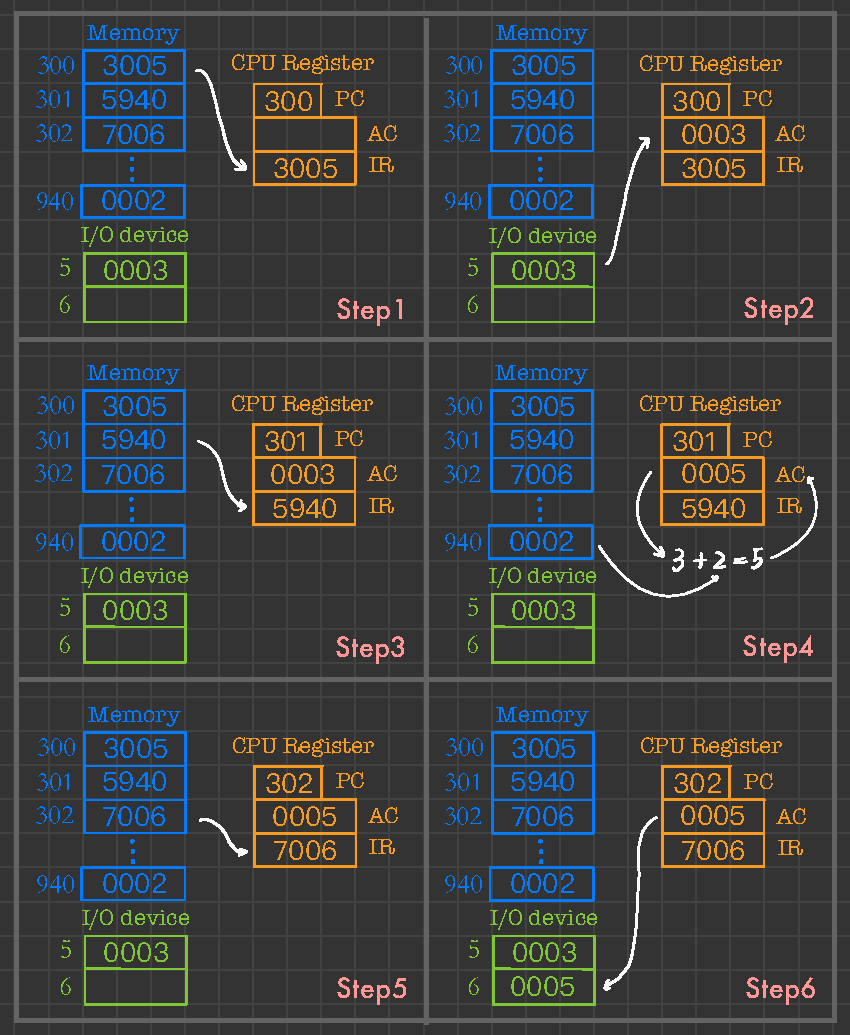
\includegraphics[width=0.7\textwidth]{pic/p1.pdf}
            \caption{P131 3.1}
        \end{figure}
    \end{enumerate}

\subsection*{3.2}

Useful Concepts Review: 
\begin{itemize}
    \item MAR(Memory Address Register): specify the \textbf{address} in memory for the next read or write.
    \item MBR(Memory Buffer Register): contain the \textbf{data} to be written into memory or receive the data read from memory.
\end{itemize}

\begin{figure}[H]
    \centering
    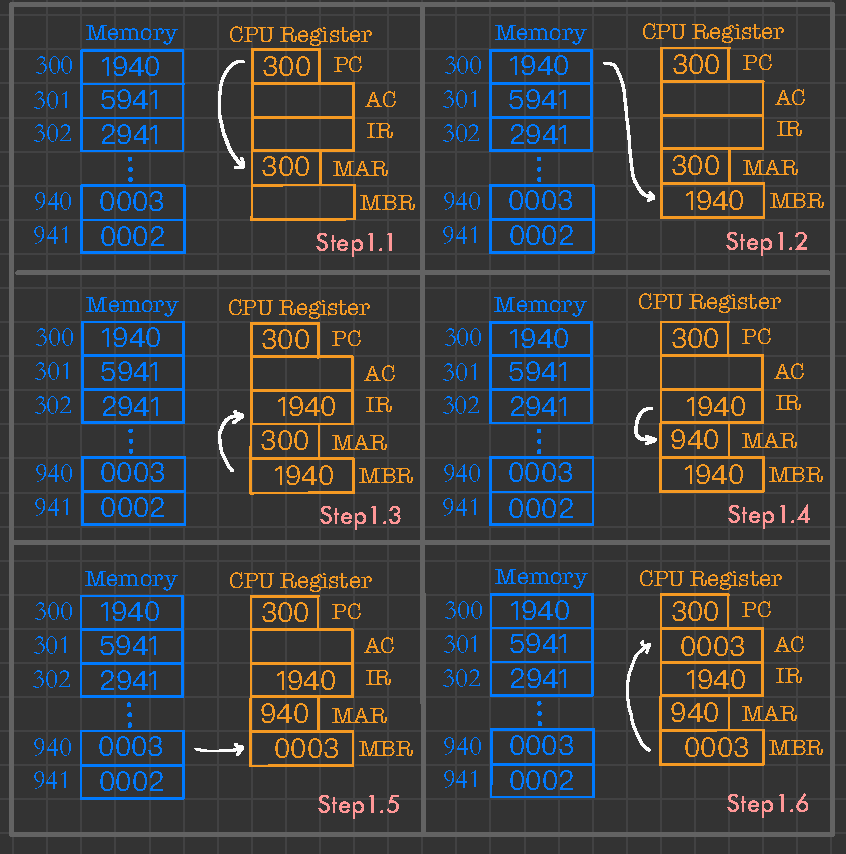
\includegraphics[width=0.5\textwidth]{pic/p2/p2-1.pdf}
    \caption{P131 3.2.1}
\end{figure}

\begin{figure}[H]
    \centering
    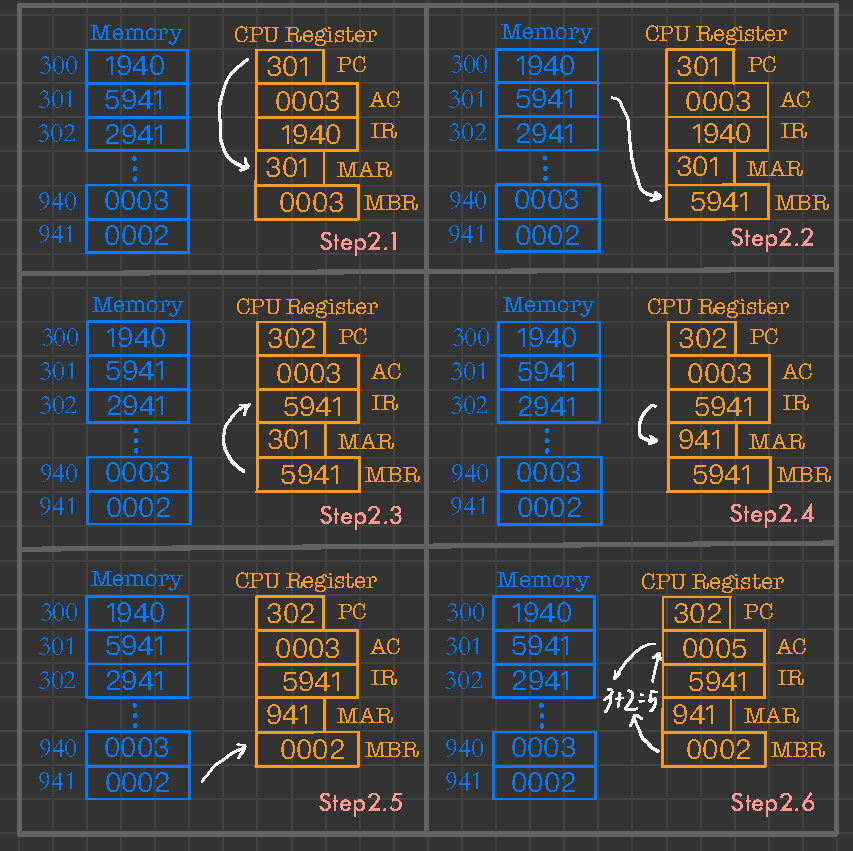
\includegraphics[width=0.5\textwidth]{pic/p2/p2-2.pdf}
    \caption{P131 3.2.2}
\end{figure}

\begin{figure}[H]
    \centering
    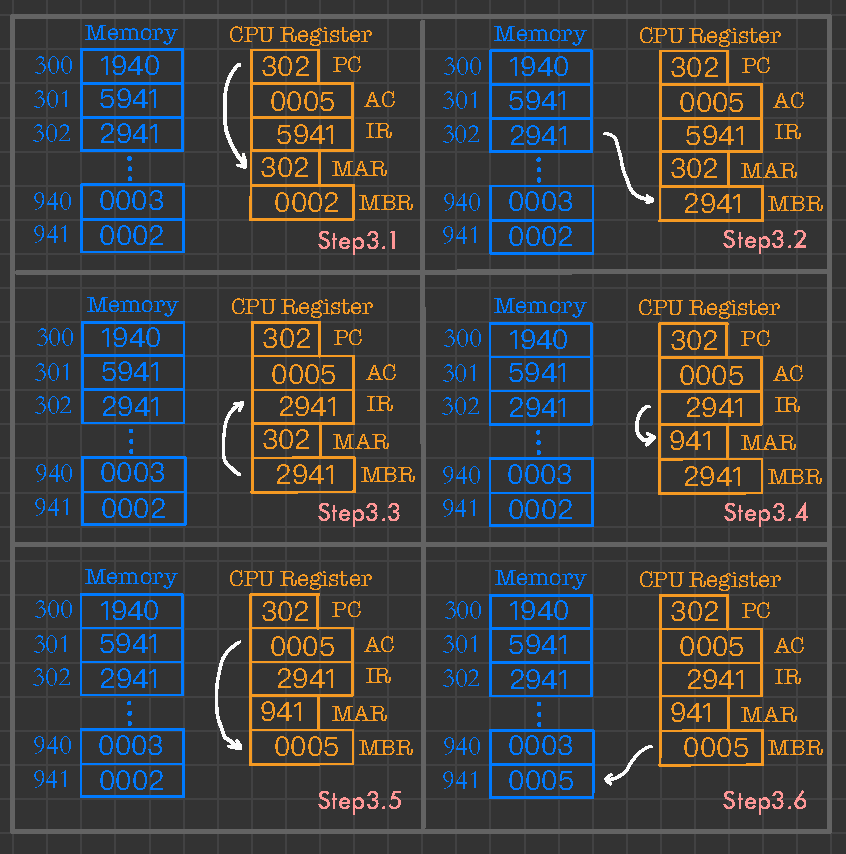
\includegraphics[width=0.5\textwidth]{pic/p2/p2-3.pdf}
    \caption{P131 3.2.3}
\end{figure}

\subsection*{3.12}
    $ T = \dfrac{1}{8\times 10^6\text{Hz}} = 125 \text{ns}$

\subsubsection*{a.}

    Answer: \textbf{2}
    $$
    \left \lceil \frac{180}{125}  \right \rceil = 2.
    $$

\subsubsection*{b.}


\section*{Other things}

\begin{itemize}
    \item \LaTeX \space code refer to these things and was complied on texlive2020.
    \begin{itemize}
        \item  \href{https://www.eecs70.org/assets/misc/homework_template.tex}{UCB-CS70's given homework template.} 
        \item  \href{https://www.latexlive.com}{A free website useful to edit \LaTeX \space formula code.}
    \end{itemize}
    \item The figures in this homework is made with \href{https://apps.apple.com/us/app/goodnotes-5/id1444383602}{GoodNotes5}.
\end{itemize}
%% The purpose of writing in English is to adapt to bilingual teaching and to improve my poor English 
%% writing skills in preparation for a possible future exchange program. 

    Thanks for your correcting and grading :).

\end{document}